\documentclass[11pt]{article}
\usepackage[T1]{fontenc}
\usepackage[utf8]{inputenc}
\usepackage{lmodern}
\usepackage[margin=1in]{geometry}
\usepackage{amsmath}
\usepackage{booktabs}
\usepackage{graphicx}
\usepackage{xcolor}
\usepackage[numbers,sort&compress]{natbib}
\usepackage[colorlinks=true,linkcolor=blue!50!black,citecolor=blue!50!black,urlcolor=blue!50!black]{hyperref}
\usepackage{caption}
\usepackage{float}
\captionsetup{font=small,labelfont=bf,labelsep=period}
\graphicspath{{figures/}}

\title{Within-Building Dependence, Target Leakage and Data Vintages in Building Energy Prediction from Public Benchmarking Data\\[6pt]\large Evidence from Seattle, 2015 to 2025}
\author{Khoty Wolie\\Independent researcher\\\texttt{khotywolie@gmail.com}}
\date{Preprint, October 2026}

\begin{document}
\maketitle

\begin{abstract}
Public building energy benchmarking disclosures are increasingly used to train machine-learning models that estimate the energy use and greenhouse-gas (GHG) emissions of buildings. We study three choices that such studies rarely report, namely how predictive performance is evaluated, which information would actually be available at prediction time, and which release (vintage) of the public data is used. We analyse Seattle's non-residential disclosure panel (15{,}621 building-years from 1{,}667 buildings, 2015 to 2025) and two releases of the 2016 data, following a protocol fixed before any model was fitted. First, because each building reappears every year with identical or near-identical attributes, row-random cross-validation underestimates the error on unseen buildings by a factor of about 2.7 for a random forest (mean absolute error on the log scale, MAE, 0.20 versus 0.53) and 2.3 for gradient boosting. It also reverses the ranking of models, and forward-temporal splits that reuse the same buildings retain most of this optimism. Second, the ENERGY STAR score, which is computed from the building's own metered energy, lowers the error by 0.127 and must be treated as target leakage rather than as a predictive feature. Third, the current consolidated release revises the reported GHG emissions of 90\% of the buildings for reporting year 2016 and holds floor areas and floor counts constant across all eleven years. With the revised GHG target the reported error rises by 0.029 (95\% CI $[0.015, 0.043]$), yet a naive baseline worsens by the same amount and the relative skill and ranking of models do not change. Absolute accuracy figures are therefore not comparable across data vintages. We close with a short reporting checklist for studies built on benchmarking data.
\end{abstract}

\section{Introduction}
\label{sec:intro}

Building energy benchmarking and disclosure ordinances now oblige owners of large buildings in many cities to report their annual energy use, and the resulting open datasets have become a common testbed for data-driven energy estimation \cite{kontokosta2017citywide,papadopoulos2019grading,amasyali2018review}. Seattle's disclosure data alone have supported gradient-boosting and explainable-AI studies of energy use and emissions \cite{pan2020data,zhang2023xai,zhang2023gtwr}, urban building energy models enriched with remote-sensing data \cite{worthy2025eo}, multi-city graph-learning estimates of operational carbon \cite{yap2025revealing} and, most recently, a multi-city benchmark for building-level emission prediction \cite{duan2026ghgbench}.

Three methodological choices strongly condition what such studies can claim, yet they are rarely made explicit. The first is the evaluation design. Benchmarking data form a panel in which the same building appears every year, so random row-level splits place the same building on both sides of the train/test boundary, a well-known source of optimism for structured data \cite{roberts2017cv,kaufman2012leakage,kapoor2023leakage}. The second is the availability of information. Some disclosed fields, such as the ENERGY STAR score or the energy-use intensity (EUI), are computed from the very metered energy that a model is meant to predict \cite{epa2021energystarscore}. The third is the data vintage. Open benchmarking portals are living datasets in which annual releases are consolidated, re-processed and sometimes restated, so two studies that both use ``Seattle 2016'' may not analyse the same numbers.

This paper quantifies the three effects on a single, well-documented city panel. Data, information tiers, splits, models, metrics, primary contrasts and decision thresholds were fixed and frozen in a protocol before any model was fitted. The contributions are as follows.
\begin{enumerate}
  \item \textbf{Evaluation design.} On an eleven-year panel we contrast row-random, building-grouped, forward-temporal and grouped-temporal evaluation. With near-identical attributes across years, random and non-grouped temporal splits mostly measure how well a learner recognises a building it has already seen, and this reverses the ranking of models (Section~\ref{sec:res-design}).
  \item \textbf{Information availability and the ENERGY STAR score.} We separate ex-ante structural information (T0), a metered baseline year (T1) and target-derived fields (T2), and show that the ENERGY STAR score, sometimes treated as non-energy metadata \cite{duan2026ghgbench}, behaves as target leakage (Section~\ref{sec:res-tiers}).
  \item \textbf{Data vintages.} We document how the current consolidated Seattle release differs from the original 2016 release and measure, with a $2\times2$ factorial design, whether the resulting change in error stems from revised targets or revised attributes, and whether it reflects a change in difficulty or only in the dispersion of the target (Section~\ref{sec:res-vintage}).
\end{enumerate}

\paragraph{Provenance.} The starting point of this research was a supervised training exercise completed by the author (CentraleSupélec and OpenClassrooms Data Scientist programme) on the 2016 Seattle file. That exercise is not part of the contribution. We reproduced it exactly during an audit and use it only as a point of comparison (Section~\ref{sec:discussion}). The research questions, the multi-year panel, the vintage comparison, the protocol and all reported analyses are new.

\section{Related work}
\label{sec:related}

\paragraph{Machine learning on benchmarking disclosures.} Data-driven building energy prediction has been reviewed extensively \cite{amasyali2018review}. City-scale studies use disclosure data to estimate the energy use of non-reporting buildings \cite{kontokosta2017citywide}, to build energy-performance grades \cite{papadopoulos2019grading,arjunan2022beem} and to analyse temporal performance patterns \cite{papadopoulos2018pattern}, and national survey data have been used to compare learners \cite{robinson2017commercial}. For Seattle, CatBoost reached $R^2=0.897$ for weather-normalised site EUI under five-fold cross-validation \cite{pan2020data}. LightGBM with SHAP explanations \cite{zhang2023xai} and spatio-temporal regression \cite{zhang2023gtwr} were used to identify drivers of energy use and emissions, and microclimate variables derived from Earth-observation products improved urban building energy models \cite{worthy2025eo}. Multi-city studies pooled up to twelve U.S.\ cities \cite{li2024generalized} or five cities on three continents with graph neural networks \cite{yap2025revealing}. GHGbench \cite{duan2026ghgbench} harmonises 491{,}591 building-year records from 26 metropolitan areas, including Seattle, and evaluates building-grouped, row-random, leave-one-city-out and temporal splits. The Seattle studies whose protocol we could verify use random splits \cite{pan2020data,yap2025revealing}. Whether these splits keep buildings disjoint depends on whether several reporting years were pooled, which is not stated.

\paragraph{Leakage and evaluation design.} Leakage occurs when information unavailable at prediction time enters training or evaluation \cite{kaufman2012leakage}. Kapoor and Narayanan \cite{kapoor2023leakage} catalogue its forms across scientific fields. A recent large-scale study finds that preprocessing leakage, such as fitting a scaler on all rows, is negligible in practice, whereas selection and boundary leakage matter \cite{roth2026leakagetypes}. For grouped, spatial or temporal data, blocked or grouped validation is recommended \cite{roberts2017cv,bergmeir2012cvts}, together with nested model selection \cite{varma2006bias}.

\paragraph{The ENERGY STAR score.} The score is a percentile rank obtained from a look-up table applied to the ratio of a property's actual source EUI to the source EUI predicted by an EPA regression, and it requires twelve months of metered data for all fuels \cite{epa2021energystarscore}. Its regression models and its uncertainty have been criticised \cite{scofield2014energystar,hsu2014selfreported}, and machine-learning alternatives to the underlying regressions have been proposed \cite{arjunan2020energystarpp}. For given operating characteristics the score is a monotone function of the measured source EUI, so using it as an input to predict energy use leaks the target.

\paragraph{Data vintages.} Macroeconomics has long distinguished ``real-time'' data vintages from later revised data when evaluating forecasts \cite{croushore2001realtime}, and dataset documentation practices recommend recording the version of every dataset used \cite{gebru2021datasheets}. We are not aware of an analysis of release revisions in building benchmarking data, and none of the studies above reports which release of the data it used.

\section{Research questions and hypotheses}
\label{sec:rq}

\textbf{RQ1.} How much does the evaluation design change the estimated performance? \textbf{RQ2.} What is the value of the information actually available in each use case, and how much of the apparent value of the ENERGY STAR score is leakage? \textbf{RQ3.} Does the release of the public data change measured performance and comparative conclusions?

The protocol states eight primary contrasts (P1 to P8, Table~\ref{tab:contrasts}) with Holm correction and a practical threshold. An effect is called \emph{substantial} only if its Holm-adjusted test is significant at the 5\% level \emph{and} $|\Delta\mathrm{MAE}|\ge0.02$ on the log scale, which corresponds to about 2\% relative error. The hypotheses are H1, grouped error exceeds row-random error (P1, P2); H2, error grows with the forecast horizon (P3); H3, a complex learner does not clearly beat Ridge on unseen buildings (P4); H4, error is heterogeneous across building groups (descriptive); H5, adding the ENERGY STAR score strongly lowers error, a gain classified \emph{a priori} as leakage (P5); HV1, revisions change error, more for GHG, which was heavily revised, than for energy (P6, P7); and HV2, as-of versus snapshot attributes change error at a fixed target (P8). The protocol designated the vintage question as primary. We present it last because the evaluation-design effects proved much larger, and the codes P1 to P8 are those of the protocol. Three analyses (X1 to X3) were added after the primary results and are reported as exploratory.

\section{Data and methodology}
\label{sec:methods}

\subsection{Data releases and population}
We use the consolidated dataset ``Building Energy Benchmarking Data, 2015--Present'' published by the City of Seattle \cite{seattle2026benchmarking}, downloaded on 29 October 2026 (public domain, with its SHA-256 hash recorded and checked at every run). We also use the original 2016 annual release \cite{seattle2016benchmarking_original}, which the city portal no longer serves. The copy used was authenticated against five summary statistics recorded in the original training notebooks. The analysis population is defined from metadata only (Appendix Table~\ref{tab:attrition}) and keeps non-residential buildings with compliant reports, not demolished, and with positive site energy. No observation is removed on the basis of the target distribution. The result is 15{,}621 building-years from 1{,}667 buildings, with 1{,}336 to 1{,}521 buildings per year. The primary target is $y=\log(\text{site energy in kBtu})$ and $\log(\text{GHG emissions})$ is secondary.

\subsection{Information tiers}
\textbf{T0 (ex ante)} contains what is known about a building that has never reported energy, namely log floor areas, parking share, largest-use share, floors, number of buildings, year built, coordinates, building type, EPA property type (15 types plus a grouped class for types with fewer than 30 buildings) and neighbourhood. \textbf{T1 (metered baseline)} adds the fuel shares and the log energy of the building's first observed year strictly before the target year, capped at the training cut-off in temporal designs. This corresponds to the use case of the original exercise. \textbf{T2 (target-derived)} contains same-year fields computed from the target's own meter data, namely the ENERGY STAR score, site and source EUI, GHG intensity and the per-fuel consumptions, whose sum equals the target (median ratio 1.000). T2 is used only to quantify leakage.

\subsection{Evaluation designs}
Design S1 is a row-random 5-fold cross-validation (CV) over building-years with 5 repeats, and S2 a building-grouped 5-fold CV with 5 repeats. Design S3 is forward temporal, training on years $\le t$ and testing on year $t+h$ for $t\in\{2017,\dots,2024\}$ and $h\in\{1,2,3\}$. Design S4 restricts S3 to test buildings never seen in training. Hyperparameters are tuned by nested 3-fold CV inside each training fold, random in S1 to mirror common practice and building-grouped otherwise \cite{varma2006bias}.

\subsection{Models}
M0 predicts the median of $y$ by property type. M1 is persistence, the log energy of the most recent prior year, and applies to T1 only. M2 is Ridge regression, M3 a random forest with 500 trees and M4 histogram gradient boosting. All hyperparameter grids were fixed in advance. Preprocessing (median imputation, one-hot encoding and, for Ridge, scaling) is fitted on training folds only.

\subsection{Metrics and inference}
The primary metric is the MAE of $y$ on the log scale, which can be read as a typical relative error. Secondary metrics are the RMSE, $R^2$, the median absolute percentage error and the MAE in kBtu with Duan's smearing correction \cite{duan1983smearing}. Uncertainty is estimated with a cluster bootstrap over buildings with $B=2000$ resamples \cite{field2007clustered}. Contrasts are paired on identical test rows after averaging errors over CV repeats.

\subsection{Reproducibility}
Analyses use Python 3.11 with scikit-learn 1.9.1, pandas 3.1 and NumPy 2.4 on a 24-core CPU, and all experiments together take about 75 minutes. Every run stores the frozen configuration, the data hashes, the commit identifier, the full software environment, per-row predictions and per-fold metrics. Deviations from the protocol were logged with their date and with whether results were known at the time. Unit tests cover the split invariants (no building overlap in grouped designs, no future year in training, causal baselines).

\section{Results}
\label{sec:results}

Table~\ref{tab:contrasts} summarises the eight primary contrasts in the order of the protocol.

\begin{table}[t]
\centering\small
\caption{Primary contrasts of the protocol. Differences in MAE on the log scale, with cluster-bootstrap 95\% confidence intervals and Holm-adjusted $p$-values. ``Substantial'' requires significance and $|\Delta|\ge0.02$. Gradient boosting (M4) unless stated otherwise.}
\label{tab:contrasts}
\resizebox{\linewidth}{!}{\begin{tabular}{llrcrl}
\toprule
 & Contrast (difference in MAE on the log scale) & Estimate & 95\% CI & $p_{\mathrm{Holm}}$ & Verdict \\
\midrule
P1 & Building-grouped minus row-random CV (T0) & $+0.299$ & [$+0.281$, $+0.316$] & $<0.005$ & substantial \\
P2 & Building-grouped minus row-random CV (T1) & $+0.120$ & [$+0.111$, $+0.129$] & $<0.005$ & substantial \\
P3 & Forward temporal, horizon 3 minus horizon 1 (T0) & $+0.050$ & [$+0.044$, $+0.056$] & $<0.005$ & substantial \\
P4 & Gradient boosting minus Ridge, unseen buildings and future years (T0) & $+0.016$ & [$+0.004$, $+0.029$] & 0.048 & significant, below threshold \\
P5 & T0 with ENERGY STAR minus T0, grouped CV & $-0.127$ & [$-0.140$, $-0.113$] & $<0.005$ & substantial \\
P6 & Original minus consolidated 2016 release, GHG target & $-0.029$ & [$-0.043$, $-0.015$] & $<0.005$ & substantial \\
P7 & Original minus consolidated 2016 release, energy target & $+0.005$ & [$-0.006$, $+0.016$] & 0.328 & not significant \\
P8 & As-of minus snapshot attributes, energy target & $+0.007$ & [$-0.003$, $+0.018$] & 0.328 & not significant \\
\bottomrule
\end{tabular}
}
\end{table}

\subsection{Random and non-grouped splits reward recognising seen buildings}
\label{sec:res-design}

Row-random CV yields a much lower error than building-grouped CV for tree ensembles (Table~\ref{tab:e1} and Figure~\ref{fig:e1}). The error is 0.197 versus 0.527 for the random forest and 0.224 versus 0.523 for gradient boosting (P1, $\Delta=+0.299$), whereas Ridge is almost unaffected (0.504 versus 0.514). The ranking is therefore reversed. Trees appear more than twice as accurate as Ridge under random CV, but on unseen buildings Ridge is at least as accurate as both tree ensembles. The gap persists, although smaller, when a metered baseline year is available (T1, P2, $\Delta=+0.120$).

\begin{table}[t]
\centering\small
\caption{MAE on the log scale under row-random and building-grouped cross-validation, averaged over 5 repeats.}
\label{tab:e1}
\begin{tabular}{lcccc}
\toprule
 & \multicolumn{2}{c}{T0 (15{,}621 rows)} & \multicolumn{2}{c}{T1 (13{,}954 rows)} \\
\cmidrule(lr){2-3}\cmidrule(lr){4-5}
Model & Row-random & Grouped & Row-random & Grouped \\
\midrule
Median by type & 0.903 & 0.914 & 0.902 & 0.913 \\
Ridge & 0.504 & 0.514 & 0.289 & 0.294 \\
Random forest & 0.197 & 0.527 & 0.151 & 0.298 \\
Gradient boosting & 0.224 & 0.523 & 0.184 & 0.304 \\
\bottomrule
\end{tabular}

\end{table}

\begin{figure}[t]
\centering
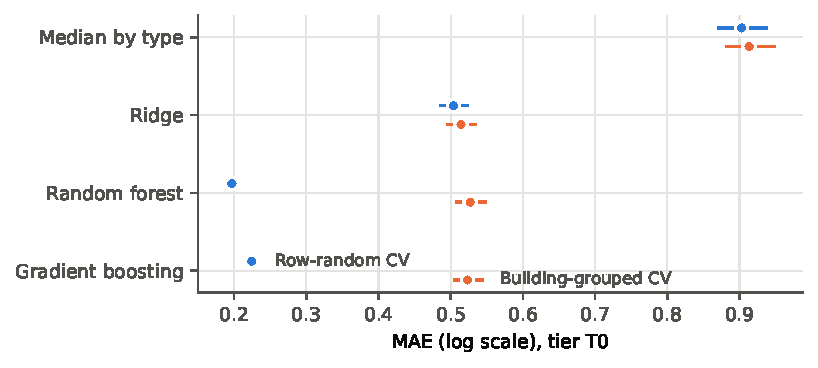
\includegraphics[width=0.8\linewidth]{fig_e1_random_vs_grouped.pdf}
\caption{Row-random versus building-grouped cross-validation for tier T0. Points show the MAE on the log scale and whiskers the 95\% cluster-bootstrap confidence intervals.}
\label{fig:e1}
\end{figure}

\begin{figure}[t]
\centering
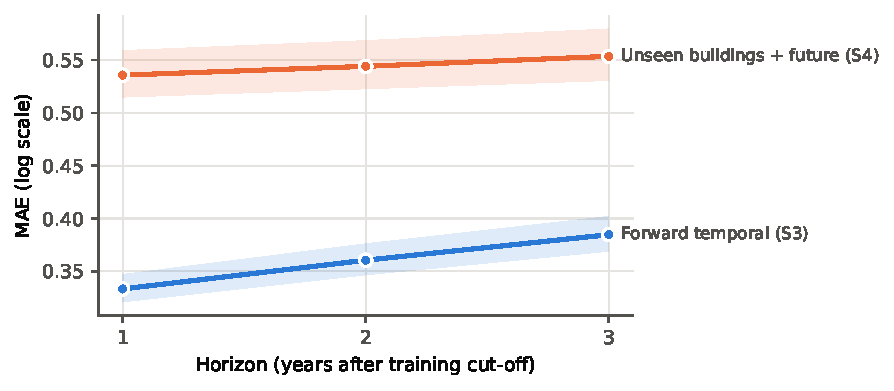
\includegraphics[width=0.75\linewidth]{fig_e2_e3_horizon.pdf}
\caption{Gradient boosting error by forecast horizon under forward-temporal evaluation with the same buildings (S3) and with unseen buildings (S4), tier T0. Bands show 95\% confidence intervals.}
\label{fig:horizon}
\end{figure}

Temporal evaluation alone does not remove the optimism (Table~\ref{tab:horizon} and Figure~\ref{fig:horizon}). With the same buildings in training and test (S3), gradient boosting reaches 0.333 to 0.385 depending on the horizon, against 0.536 to 0.554 with unseen buildings (S4). Error grows with the horizon (P3, $\Delta=+0.050$), and the test years 2020 and 2021 are harder (S3 at $h=1$, 0.357 versus 0.325 for the other years). On unseen buildings, gradient boosting is not better than Ridge (P4, $\Delta=+0.016$, significant but below the practical threshold).

\begin{table}[t]
\centering\small
\caption{MAE on the log scale by forecast horizon $h$ (years after the training cut-off), averaged over the cut-offs 2017 to 2024.}
\label{tab:horizon}
\begin{tabular}{llcccccc}
\toprule
 & & \multicolumn{3}{c}{Forward temporal (S3)} & \multicolumn{3}{c}{Unseen buildings + future (S4)} \\
\cmidrule(lr){3-5}\cmidrule(lr){6-8}
Tier & Model & $h=1$ & $h=2$ & $h=3$ & $h=1$ & $h=2$ & $h=3$ \\
\midrule
T0 & Median by type & 0.909 & 0.916 & 0.923 & 0.922 & 0.929 & 0.938 \\
T0 & Ridge & 0.510 & 0.519 & 0.530 & 0.519 & 0.527 & 0.538 \\
T0 & Random forest & 0.284 & 0.320 & 0.354 & 0.539 & 0.546 & 0.556 \\
T0 & Gradient boosting & 0.333 & 0.360 & 0.385 & 0.536 & 0.544 & 0.554 \\
\midrule
T1 & Persistence (last year) & 0.174 & 0.248 & 0.298 & 0.174 & 0.248 & 0.298 \\
T1 & Ridge & 0.313 & 0.335 & 0.365 & 0.317 & 0.339 & 0.369 \\
T1 & Random forest & 0.223 & 0.264 & 0.296 & 0.324 & 0.341 & 0.358 \\
T1 & Gradient boosting & 0.244 & 0.278 & 0.308 & 0.338 & 0.355 & 0.375 \\
\bottomrule
\end{tabular}

\end{table}

\paragraph{Exploratory analysis X1.} Each of the 1{,}667 buildings has a unique T0 attribute vector, so the attributes form an exact fingerprint. To test whether flexible learners rely on exact identification, X1 re-runs S1 and S2 with continuous attributes perturbed independently on every row (floor areas multiplied by $1+\varepsilon$ with $\varepsilon\sim\mathcal{N}(0,0.02)$, coordinates shifted by $\mathcal{N}(0,0.002^\circ)$ and year built shifted by up to two years). We expected a strong rise of the row-random error of tree ensembles. The rise is real but moderate (Table~\ref{tab:x1}), from 0.197 to 0.240 for the random forest and from 0.225 to 0.288 for gradient boosting. Both values remain far below the grouped error with perturbed attributes (0.528 and 0.521), and Ridge and all grouped results are unchanged. Exact identification therefore explains only part of the optimism. Near-identical attributes are enough for a flexible learner to match a building with its own records from other years, and that building's consumption is highly persistent (year-to-year correlation of log energy between 0.94 and 0.98). The relevant mechanism is within-building dependence, which only grouping removes.

\begin{table}[t]
\centering\small
\caption{Exploratory analysis X1. MAE on the log scale with exact and with row-wise perturbed continuous attributes (2 repeats of 5 folds, tier T0).}
\label{tab:x1}
\begin{tabular}{lcccc}
\toprule
 & \multicolumn{2}{c}{Exact attributes} & \multicolumn{2}{c}{Jittered attributes} \\
\cmidrule(lr){2-3}\cmidrule(lr){4-5}
Model & Row-random & Grouped & Row-random & Grouped \\
\midrule
Ridge & 0.504 & 0.513 & 0.504 & 0.513 \\
Random forest & 0.197 & 0.530 & 0.240 & 0.528 \\
Gradient boosting & 0.225 & 0.522 & 0.288 & 0.521 \\
\bottomrule
\end{tabular}

\end{table}

\subsection{Information tiers and ENERGY STAR leakage}
\label{sec:res-tiers}

On the rows where a score is reported (Table~\ref{tab:e5} and Figure~\ref{fig:e5}), adding the ENERGY STAR score to T0 lowers the grouped-CV error of gradient boosting from 0.450 to 0.323 (P5, $\Delta=-0.127$). This is close to the gain brought by a genuine metered baseline year (T1 reaches 0.282 on the subset of these rows that have a baseline), and the score still adds to T1 (0.242). Same-year EUI, an upper bound for target leakage, yields 0.077. Following the rule fixed before the experiments, the ENERGY STAR gain is attributed to leakage, because for given operating characteristics the score is a monotone function of the measured source EUI \cite{epa2021energystarscore}. The score is only reported for eligible property types with complete data, so this comparison is restricted to those rows (66\% of building-years in S2) and does not describe the remaining buildings.

\begin{table}[t]
\centering\small
\caption{MAE on the log scale by information tier, on rows with a reported ENERGY STAR score (10{,}363 building-years in S2).}
\label{tab:e5}
\begin{tabular}{lcccc}
\toprule
 & \multicolumn{2}{c}{Grouped CV (S2)} & \multicolumn{2}{c}{Unseen + future (S4)} \\
\cmidrule(lr){2-3}\cmidrule(lr){4-5}
Information tier & Ridge & Gr.\ boosting & Ridge & Gr.\ boosting \\
\midrule
T0 (structural) & 0.441 & 0.450 & 0.452 & 0.461 \\
T0 + ENERGY STAR & 0.328 & 0.323 & 0.327 & 0.332 \\
T1 (T0 + baseline year) & 0.271 & 0.282 & 0.307 & 0.316 \\
T1 + ENERGY STAR & 0.238 & 0.242 & 0.268 & 0.275 \\
T0 + same-year EUI (leakage ceiling) & 0.373 & 0.077 & 0.384 & 0.087 \\
\bottomrule
\end{tabular}

\end{table}

\begin{figure}[t]
\centering
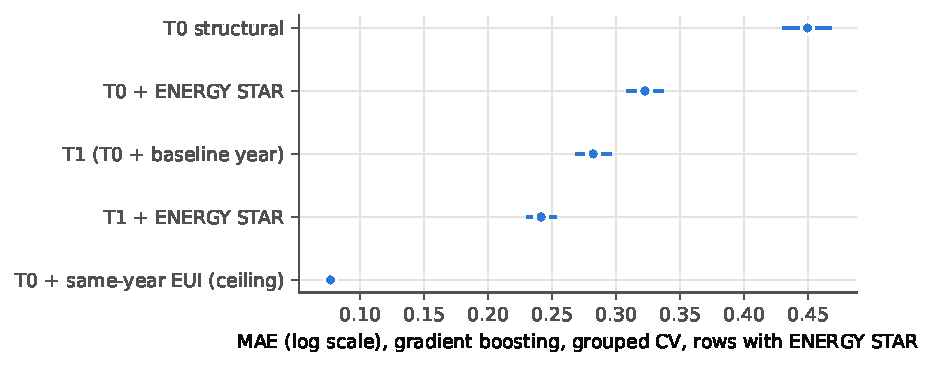
\includegraphics[width=0.75\linewidth]{fig_e5_energy_star_leakage.pdf}
\caption{Information tiers and ENERGY STAR leakage for gradient boosting under building-grouped cross-validation, on rows with a reported score. Whiskers show 95\% confidence intervals.}
\label{fig:e5}
\end{figure}

In the metered-baseline use case, a baseline year helps substantially. For Ridge on unseen buildings and future years, the error falls from 0.522 with T0 to 0.326 with T1, on nearly identical row sets of 11{,}495 and 11{,}294 building-years. Simple persistence of the most recent year (M1) is nevertheless more accurate than every learner (0.174 at $h=1$).

\paragraph{Exploratory analysis X2.} Persistence uses the most recent year whereas T1 uses the first observed year, so the comparison above is not made at equal information. In X2 the T1 baseline is redefined as the most recent observed year before the target, capped at the cut-off for test rows, which is exactly the information used by persistence. Learners still do not beat persistence on unseen buildings and future years (Table~\ref{tab:x2}). Over all horizons, persistence reaches 0.234, gradient boosting 0.254 and Ridge 0.258, and at $h=1$ the values are 0.174, 0.194 and 0.186. Once a recent metered year is known, the learners using structural attributes did not improve on persistence in this panel.

\begin{table}[t]
\centering\small
\caption{Exploratory analysis X2. T1 with the most recent prior year as baseline, on unseen buildings and future years (S4). MAE on the log scale.}
\label{tab:x2}
\begin{tabular}{lcccc}
\toprule
Model (T1 with last-year baseline, S4) & $h=1$ & $h=2$ & $h=3$ & All \\
\midrule
Persistence (last year) & 0.174 & 0.248 & 0.298 & 0.234 \\
Ridge & 0.186 & 0.269 & 0.344 & 0.258 \\
Gradient boosting & 0.194 & 0.272 & 0.314 & 0.254 \\
\bottomrule
\end{tabular}

\end{table}

\subsection{Data revisions change error levels, not model skill or ranking}
\label{sec:res-vintage}

Table~\ref{tab:vintage} compares the 3{,}194 buildings present in both releases of 2016. The consolidated release reports different GHG emissions for 90.4\% of them (median ratio of consolidated to original values 0.945, 25th percentile 0.833), different total floor areas for 9.5\% and a different building type for 9.6\%. In addition, 182 buildings appear only in the original release and 59 only in the consolidated one. Within the consolidated panel, total floor area, floors and building and parking areas never change across the eleven years for any building observed more than once, whereas the largest-use floor area changes for 58.7\% of them. Structural attributes are therefore a single snapshot applied to all years.

\begin{table}[t]
\centering\small
\caption{Revisions between the original 2016 release and the 2016 records of the consolidated release, for buildings matched on their identifier.}
\label{tab:vintage}
\begin{tabular}{lrr}
\toprule
Field (reporting year 2016) & Buildings compared & Share revised \\
\midrule
Total GHG emissions & 3,179 & 90.4\% \\
Parking floor area & 3,194 & 18.2\% \\
Building type & 3,194 & 9.6\% \\
Total floor area & 3,194 & 9.5\% \\
Number of buildings & 3,187 & 6.3\% \\
ENERGY STAR score & 2,415 & 4.3\% \\
Site energy use & 3,178 & 1.9\% \\
Largest-use floor area & 3,175 & 1.7\% \\
Number of floors & 3,194 & 0.5\% \\
Year built & 3,194 & 0.1\% \\
\bottomrule
\end{tabular}
% GHG ratio consolidated/original quantiles: p05=0.825, p25=0.833, median=0.945, p95=0.994

\end{table}

\begin{figure}[t]
\centering
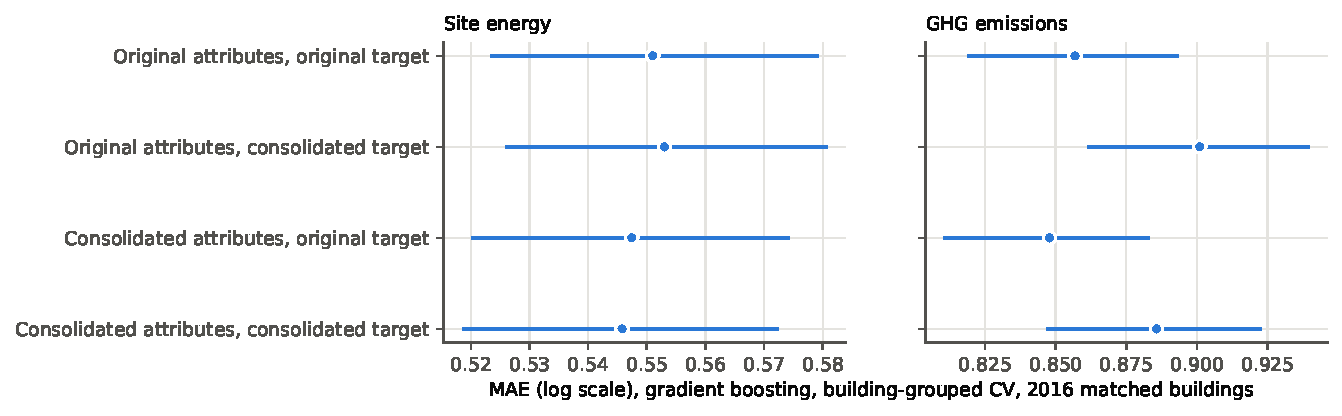
\includegraphics[width=\linewidth]{fig_e6_vintage_factorial.pdf}
\caption{The same protocol applied to two releases of 2016 (1{,}343 matched buildings, 1{,}341 for GHG). Gradient boosting under building-grouped cross-validation, MAE on the log scale with 95\% cluster-bootstrap confidence intervals. Rows combine the release of the attributes with the release of the target.}
\label{fig:e6}
\end{figure}

Applying the same protocol to both releases (Table~\ref{tab:e6} and Figure~\ref{fig:e6}), the GHG error is lower with the original release than with the consolidated one (P6, $\Delta=-0.029$, substantial). The factorial design attributes the difference to the target. Holding the consolidated attributes fixed, switching only the target release changes the error by $-0.038$ (95\% CI $[-0.044,-0.031]$), while switching only the attributes changes it by $+0.015$ (95\% CI $[0.002,0.029]$, unadjusted and secondary). For site energy, which was revised for only 1.9\% of buildings, neither the release (P7) nor the attributes (P8) has a measurable effect. In all cells the ordering of models is identical (Spearman rank correlation of 1.0 for both targets).

\begin{table}[t]
\centering\small
\caption{2016 vintage factorial. MAE on the log scale under building-grouped cross-validation for each combination of attribute release and target release.}
\label{tab:e6}
\begin{tabular}{llcccc}
\toprule
 & & \multicolumn{2}{c}{Site energy} & \multicolumn{2}{c}{GHG emissions} \\
\cmidrule(lr){3-4}\cmidrule(lr){5-6}
Attributes & Target & Ridge & Gr.\ boosting & Ridge & Gr.\ boosting \\
\midrule
original & original & 0.545 & 0.551 & 0.852 & 0.857 \\
original & consolidated & 0.545 & 0.553 & 0.896 & 0.901 \\
consolidated & original & 0.538 & 0.547 & 0.844 & 0.848 \\
consolidated & consolidated & 0.535 & 0.546 & 0.885 & 0.886 \\
\bottomrule
\end{tabular}

\end{table}

\paragraph{Exploratory analysis X3.} During internal review we asked whether the revised GHG target is genuinely harder to predict or merely more dispersed. The revised log-GHG target has a larger standard deviation (1.578 versus 1.541), and the naive median-by-type baseline worsens by the same amount as gradient boosting (Table~\ref{tab:x3}). Relative to that baseline, the skill of gradient boosting is unchanged, with an MAE ratio of 0.781 for the original release and 0.787 for the consolidated one (paired difference $-0.006$, 95\% CI $[-0.018, 0.007]$). The revision thus changes the absolute level of the error but not the skill or the ranking of the models. Absolute accuracy figures obtained on different vintages are not comparable, whereas relative conclusions were robust here.

\begin{table}[t]
\centering\small
\caption{Exploratory analysis X3. Target dispersion and skill relative to the naive baseline in the 2016 vintage factorial (gradient boosting, building-grouped cross-validation).}
\label{tab:x3}
\begin{tabular}{llrrrr}
\toprule
Target & Release & SD of $\log y$ & MAE naive & MAE boosting & Ratio \\
\midrule
Site energy & original & 1.342 & 0.937 & 0.551 & 0.588 \\
Site energy & consolidated & 1.338 & 0.936 & 0.546 & 0.583 \\
\multicolumn{5}{r}{Paired difference, original minus consolidated [95\% CI]} & $+0.005$ [$-0.006$, $+0.017$] \\
\midrule
GHG emissions & original & 1.541 & 1.097 & 0.857 & 0.781 \\
GHG emissions & consolidated & 1.578 & 1.126 & 0.886 & 0.787 \\
\multicolumn{5}{r}{Paired difference, original minus consolidated [95\% CI]} & $-0.006$ [$-0.018$, $+0.007$] \\
\bottomrule
\end{tabular}

\end{table}

\subsection{Heterogeneity}
On unseen buildings, errors vary by a factor of more than two across property types (Figure~\ref{fig:e4}).

\begin{figure}[t]
\centering
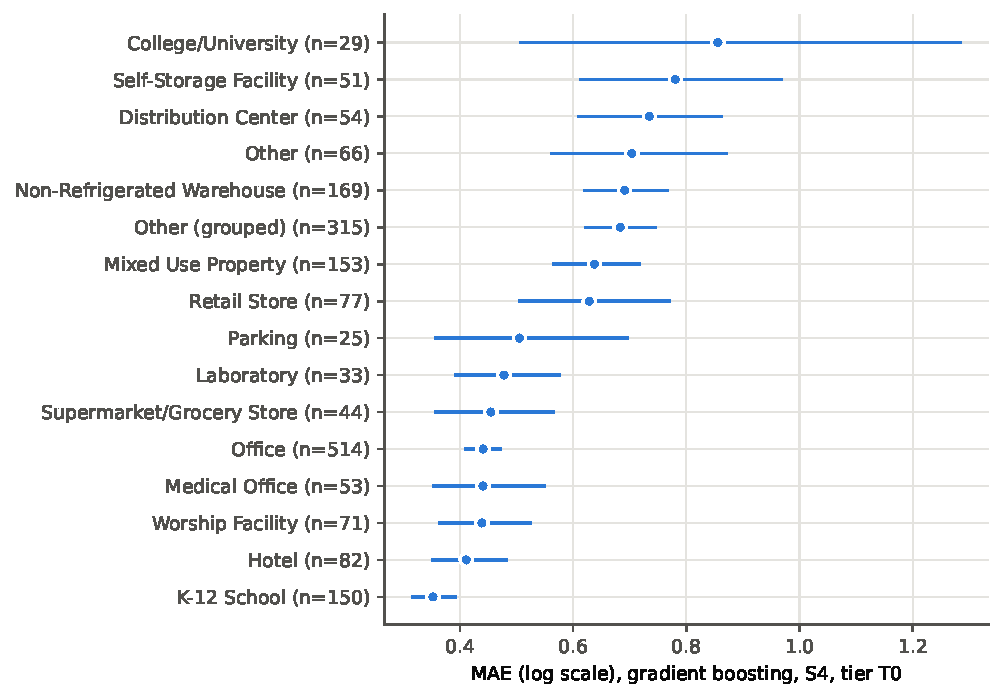
\includegraphics[width=0.75\linewidth]{fig_e4_heterogeneity_property_type.pdf}
\caption{Error by property type on unseen buildings and future years (design S4, tier T0, gradient boosting). The number of buildings is given in brackets; whiskers show 95\% confidence intervals.}
\label{fig:e4}
\end{figure} K-12 schools are the easiest (0.352), while colleges, self-storage facilities, distribution centres and warehouses are the hardest (0.69 to 0.86). Error decreases with size, from 0.640 in the smallest floor-area quintile to 0.490 in the largest, and it is highest in the industrial Greater Duwamish area (0.626).

\section{Discussion}
\label{sec:discussion}

\paragraph{Within-building dependence drives the optimism.} When attributes do not change over time, a building's records in different years are near-duplicates in attribute space, and its consumption is highly persistent. Any split that places the same building in training and test lets flexible learners recover its consumption from its other years. Linear models cannot exploit this locality, which explains why random CV inflates tree ensembles but not Ridge, and why non-grouped temporal splits remain optimistic. Perturbing the attributes (X1) removes only part of the effect, so exact identification is not required, and the remedy is to group by building rather than to obfuscate attributes. For the use case that motivates many benchmarking studies, estimating buildings that have never reported \cite{kontokosta2017citywide}, only building-grouped and ideally grouped-temporal evaluation is relevant. GHGbench uses building-grouped splits for its main results \cite{duan2026ghgbench}. From the sections we read, we could not determine whether its temporal hold-out also groups buildings, and our results suggest that this choice matters.

\paragraph{The ENERGY STAR score is not metadata.} The score requires twelve months of metered energy and is derived from the ratio of actual to predicted source EUI \cite{epa2021energystarscore}. Any model that uses it to predict energy use or emissions therefore benefits from the target. Treating the score as clean metadata, as in the original training exercise and in at least one recent benchmark tier \cite{duan2026ghgbench}, overstates deployable accuracy.

\paragraph{What a public benchmarking dataset measures depends on its release.} The consolidated Seattle release is not a stack of annual snapshots. GHG emissions have been restated, and structural attributes reflect a single, recent state of each building. We cannot attribute the revisions to a specific cause because no documentation was found, but their consequences are measurable. For an outcome that was heavily revised, such as GHG emissions, the absolute error that a study reports depends on the release, because the revision changed the dispersion of the target. Skill relative to a naive baseline and the comparison between models were stable in our setting. Absolute accuracy figures should therefore be compared across studies only when they use the same vintage, or be accompanied by a baseline-relative measure. Studies should also report the release, download date and checksum of the data they use, as is standard for real-time macroeconomic data \cite{croushore2001realtime,gebru2021datasheets}.

\paragraph{Perspective on the original exercise.} The original notebook reported a test $R^2$ of 0.53 for a linear regression evaluated on a single random split after truncating the largest consumers, a result we reproduced exactly. Under our protocol on the same 2016 release, Ridge reaches $R^2=0.668\pm0.045$. The two figures are not comparable, because truncating the largest consumers reduces the variance of the target and therefore $R^2$. This is one reason for reporting MAE as the primary metric.

\paragraph{Recommendations.} For studies that train models on benchmarking disclosures, we recommend to
\begin{enumerate}
  \item pin and report the data release, with its download date and checksum;
  \item state the use case and the information tier, and exclude target-derived fields such as EUI, per-fuel use and the ENERGY STAR score from deployable models;
  \item evaluate with building-grouped splits, and with grouped-temporal splits for forecasting claims;
  \item report errors on the original scale and by building type, together with a naive baseline and, when past consumption is available, a persistence baseline, so that results remain interpretable across data vintages.
\end{enumerate}

\section{Limitations and threats to validity}
\label{sec:limitations}
This study covers a single city. The magnitude of the effects may differ elsewhere, although the mechanisms involved (within-building dependence, score construction and data revisions) are generic. Only two releases of one reporting year could be compared, because other vintages are no longer served by the portal, and the causes of the revisions are undocumented. The two 2016 releases differ in population, so the vintage experiment is restricted to matched buildings, and the attribute-snapshot effect (P8) was tested on a cross-section only. EPA property types change for 19.7\% of multi-year buildings and were treated as annual attributes. The Duan correction uses in-sample residuals, which is optimistic for tree ensembles, but it affects only a secondary metric. The exploratory analyses X1 to X3 were decided after the primary results (X3 during internal review) and are not covered by the multiplicity correction. Finally, the copy of the original 2016 release could be authenticated against statistics recorded in the original notebooks but not against a checksum published by the city.

\section{Conclusion}
\label{sec:conclusion}
Using Seattle's benchmarking disclosures, we showed that the evaluation design, the information available at prediction time and the release of the data each change what a model appears to achieve, in some cases more than the choice of learner. Within-building dependence made random and non-grouped temporal evaluation reward the recognition of seen buildings. The ENERGY STAR score leaked the target. Data revisions changed the dispersion of the GHG target and hence the absolute error a study would report, though not the skill or ranking of models. Simple reporting conventions would make results built on these widely used datasets comparable and honest about deployment.

\section*{Data and code availability}
The consolidated dataset is public domain and available from the City of Seattle open-data portal \cite{seattle2026benchmarking}, and the exact snapshot used is identified by its SHA-256 hash. Code, unit tests, the frozen protocol, configuration files, per-run provenance records, result tables, figure scripts and the LaTeX source of this paper are available under the MIT licence at \url{https://github.com/Khoty-WOLIE/building-energy-benchmarking-evaluation}. Per-row predictions are not stored there because the code regenerates them, and the raw data files are not redistributed.

\section*{Acknowledgements}
The author used generative AI tools as research assistants, for literature searches, programming support and text editing. The author designed the study, made all scientific decisions, verified the results and takes full responsibility for the content.

\section*{Funding and competing interests}
This work received no specific funding. The author declares no competing interests.

\bibliographystyle{plainnat}
\bibliography{references}

\appendix
\section{Supplementary material}
\begin{table}[H]
\centering\small
\caption{Construction of the analysis population (consolidated release, 2015 to 2025).}
\label{tab:attrition}
\begin{tabular}{lrr}
\toprule
Selection step (cumulative) & Building-years & Buildings \\
\midrule
All records, 2015 to 2025 & 38,309 & 3,871 \\
Non-residential buildings & 17,392 & 1,744 \\
Compliant reports & 16,126 & 1,736 \\
Not demolished & 15,865 & 1,668 \\
Site energy reported and positive & 15,621 & 1,667 \\
Total floor area positive & 15,621 & 1,667 \\
\bottomrule
\end{tabular}

\end{table}

\end{document}
